\if0
\section{C++ のラムダ関数}
\fi
\section{The Lambda Function of C++11} \label{s:lambda}

The specification of lambda function is defined in the C++ ISO standard called C++11.
From GCC version 4.5, the lambda function is supported in the C++ standard library.

ArchHDL uses the the lambda function for hardware description.
In this section, we describe about the C++11 lambda function. to the extent necessary to ArchHDL.

\begin{figure}[t]
 \lstinputlisting[language=c++]{src/def_lam.cc.part}
\caption{An example of C++ program which includes a definition of lambda function.}
 \label{src:def_lambda}
\end{figure}

\figref{src:def_lambda} shows an example of C++ program which includes a lambda function.
Note that, the program includes only the definition of a lambda function, so it has no meaning.
The 2nd line of source code is the definition of lambda function which takes two int values as arguments and returns the sum of arguments.

The description of lambda function starts from \textit{lambda-introducer} [] \footnote{
A lambda introducer may contain a \textit{lambda-capture}.
ArchHDL only uses the option [=], so we skip the details of lambda-capture at here.
}
The return type of lambda function is automatically deduced from the return expression.
In the case of \figref{src:def_lambda} line 2, the return type is deduced as int.

\begin{figure}[t]
 \lstinputlisting[language=c++]{src/ex_lam.cc}
 \caption{An example of C++ program which includes a definition of lambda function and a usage of it.}
 \label{src:ex_lambda}
\end{figure}

\figref{src:ex_lambda} shows an example of C++ program using lambda function.
As the 1st line, we need to include the \textit{functional} standard library to use lambda function.

In the 6th and 7th line, the lambda function [=](int x, int y) \{ return x + y; \} is assigned to the function object \textit{Sum}.
The type of the lambda function is std::function$<$int ()$>$, therefore \textit{Sum} is declared so.
Thus, \textit{Sum} becomes a function which takes two int arguments and returns a int value.

In the 8th line, the function \textit{Sum} is called.
The return value of \textit{Sum} is assigned to the variable \textit{c}.
The variable \textit{a} and the variable \textit{b} which they are defined in the 4th and 5th line, are given to the function \textit{Sum} as arguments.

In ArchHDL, the lambda function is used in the way like shown in the \figref{src:ex_lambda}.

\if0
C++11 と呼ばれる C++ ISO 標準により,ラムダ関数の仕様が定義された. gcc
では,バージョン 4.5 よりこの ISO 標準の一部がサポートされ,
標準ライブラリとしてラムダ関数が利用できるようになった.

我々の提案する ArchHDL では,このラムダ関数を利用する. ここでは,C++11
のラムダ関数の機能を ArchHDL のために必要な範囲で述べる.

\begin{figure}[t]
 \lstinputlisting[language=c++]{src/def_lam.cc.part}
 \caption{ラムダ関数の定義のみを含む C++ プログラムの例}
 \label{src:def_lambda}
\end{figure}

\figref{src:def_lambda} にラムダ関数の定義のみを含む C++
プログラムの例を示す. 2 行目のコードは引数に \verb`int x` と
\verb`int y` をとり,その和を返すラムダ関数の定義である.

ラムダ関数の定義は lambda-introducer と呼ばれる {[}{]} \footnote{
[] 内にキャプチャと呼ばれるラムダ関数の機能を指定する記述をする必要がある.
ArchHDL では [=] のみを使用するため説明は省略する.
} の記述からはじまる.ラムダ関数の返り値の型は, return
文より推測できる場合に省略できる.例に示したラムダ関数の返り値の型は int
と推測される.

\begin{figure}[t]
 \lstinputlisting[language=c++]{src/ex_lam.cc}
 \caption{ラムダ関数を定義して,それを使う C++ プログラムの例}
 \label{src:ex_lambda}
\end{figure}

\figref{src:ex_lambda} にラムダ関数を定義して,それを使う C++
のプログラムを示す. ラムダ関数を使うために,1 行目のように functional
という標準ライブラリをインクルードする.

6,7 行目で, 関数オブジェクト Sum に
\verb`[=](int x, int y) { return x + y; }` というラムダ関数を代入する.
このラムダ関数は int 型の値を返す関数であり,その型は
std::function\textless{}int ()\textgreater{} となる. これにより,Sum は
2 個の int 型の値を引数にとり,その和を返す関数オブジェクトとなる.

8 行目では Sum を呼び出し,返り値を変数 c に代入している. 引数には,4,
5 行目にある a, b を与えている.

ArchHDL では,ラムダ関数を \figref{src:ex_lambda}
のような使い方をしている.

\section{ArchHDL による RTL モデリング \label{ss:modeling}}

ArchHDL はハードウェアの RTL モデリングのための言語である.
Verilog HDL に近い記述方法を目指している.
ユーザはライブラリにより提供される Module クラス,reg クラス,wire クラスおよび C++11 のラムダ関数を用いて
ハードウェアを記述する.
\if0 ここ追加 \fi
\if0
gcc では,バージョン 4.5 より標準ライブラリとしてラムダ関数が利用できるのでこれ以上のバージョンを要求する.
\fi

\begin{figure}[t]
 \lstinputlisting[language=c++]{src/counter8.cc}
 \caption{ArchHDL による 8 ビットカウンタ回路の記述}
 \label{src:counter}
\end{figure}

\begin{figure}[t]
 \lstinputlisting[language=verilog]{src/counter8.v}
 \caption{Verilog HDL による 8 ビットカウンタ回路の記述}
 \label{src:counter_v}
\end{figure}

\figref{src:counter}に,ArchHDL を用いて記述した 8 ビットカウンタ回路のコードを示す.
また,\figref{src:counter_v} に,Verilog HDL で記述した 8 ビットカウンタ回路のコードを示す.
ArchHDL において,Module クラスを継承して定義されるクラス(Module 子クラス)は,
Verilog HDL におけるモジュールに相当する.
同様に reg クラス,wire クラスは,それぞれ Verilog HDL におけるレジスタ,ワイヤに相当する.

Module 子クラスは,そのメンバ関数として Init 関数および Always 関数を定義する必要がある.
これは,ライブラリにより強制されており,いずれかの関数が必要でない場合でも空の関数を定義する必要がある.

Init 関数には,モジュール内のすべてのワイヤへの継続代入の定義を記述する.
これは,Verilog HDL においてモジュール内で定義されている assign 文をすべてこの関数内に記述することに相当する.
wire クラスのインスタンスにラムダ関数を代入することでワイヤへの継続代入を記述することができる.
\figref{src:counter}では,6 行目で wire クラスの変数 out に reg クラス の counter の値を返す
ラムダ関数(\verb/[=]() { return counter(); }/)を代入している.
ここで,reg クラスのオブジェクトは関数として呼び出すことにより,そのサイクルにおける値を取得することができる.
このため,先のラムダ関数における counter() によってレジスタの値が取得できる.
これは,\figref{src:counter_v} の 6 行目に相当する.

Always 関数には,モジュール内のすべてのレジスタへのノン・ブロッキング代入を記述する.
ArchHDL では,単一クロックの立ち上がりエッジでの制御のみを対象としている.
これは,Verilog HDL における \verb/always @(posedge clock)/ ブロック内の記述に相当する.
reg クラスのインスタンスに \verb/<<=/ 演算子を用いて値を代入することでノン・ブロッキング代入を記述することができる.
ArchHDL は,演算子オーバーロードを利用して \verb/<<=/ 演算子を Verilog HDL における
ノン・ブロッキング代入に相当する値の代入として実装している.
\figref{src:counter}では,9 行目で reg クラスの変数 counter に自身の値をインクリメントした値を代入している.
これは,\figref{src:counter_v}の 8 行目に相当する.

ArchHDL では,データ型として C++ の整数型を使用している.
\figref{src:counter}の例では unsigned int 型を利用しているため,
8 ビットカウンタを実現するために値をマスクする必要がある.
reg クラスと wire クラスのオブジェクトは関数として呼び出すことにより,そのサイクルにおける値を取得することができる.


\if0
\section{ArchHDL の利点}

ArchHDL には,次に挙げる利点がある.

\begin{itemize}
 \item ハードウェアモジュール間の接続の記述が容易
 \item 論理シミュレーションが高速
\end{itemize}
ここでは特に重要な前者について述べる.

\begin{figure}[t]
 \centering
 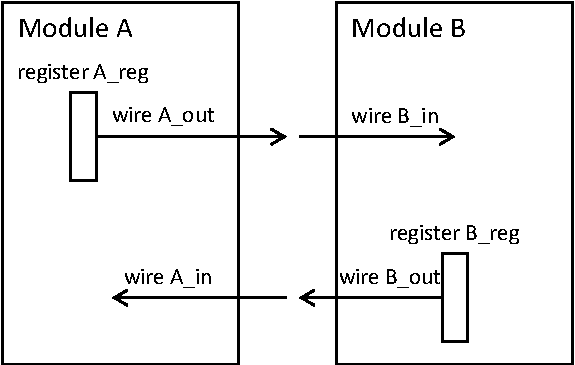
\includegraphics[clip,width=.4\textwidth]{module}
 \caption{手続き型言語では記述が難しいモジュール間の接続の例}
 \label{fig:module}
\end{figure}

\figref{fig:module} に,手続き型言語でハードウェアの挙動を記述しようとすると,
記述が難しいモジュール間の接続の例を示す.
モジュール A は入力ワイヤ A\_in,出力ワイヤ A\_out の入出力を持つ.
出力ワイヤ A\_out はレジスタ A\_reg の値を出力する.
モジュール B は入力ワイヤ B\_in,出力ワイヤ B\_out の入出力を持つ.
出力ワイヤ B\_out はレジスタ B\_reg の値を出力する.

モジュール A の出力ワイヤ A\_out は モジュール B の入力ワイヤ B\_in に接続している.
モジュール B の出力ワイヤ B\_out は モジュール A の入力ワイヤ A\_in に接続している.
モジュール A は,あるサイクルに入力として B\_reg の値を受け,A\_reg の値を出力するというモジュールである.
同様に,モジュール B は,あるサイクルに入力として A\_reg の値を受け,B\_reg の値を出力するというモジュールである.

\begin{figure}[t]
 \begin{center}
  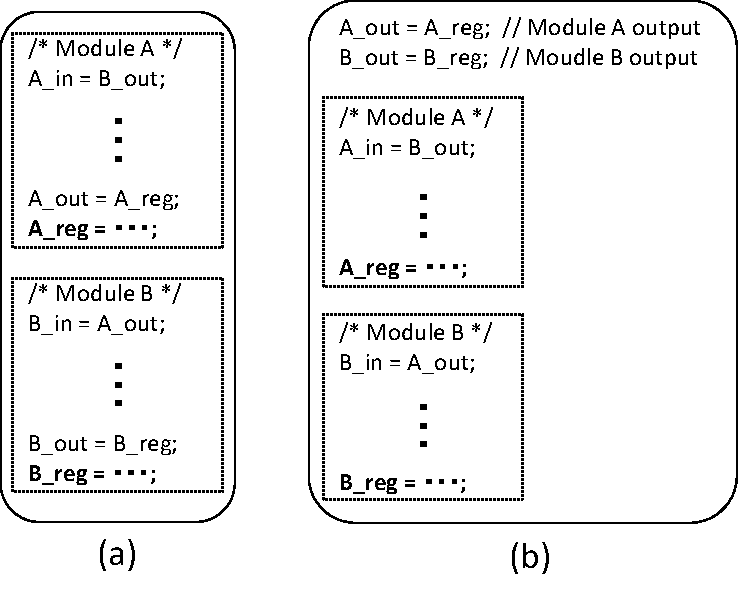
\includegraphics[width=.4\textwidth,clip]{module2}
  \caption{\figref{fig:module} のハードウェアの記述例}
  \label{fig:module2}
 \end{center}
\end{figure}

このハードウェアの挙動をモジュールごとに記述すると,\figref{fig:module2}(a)のようになる.
この記述は,
モジュールへの入力,モジュール内の処理,モジュールからの出力,レジスタの更新という
まとまりのある記述になっている.
レジスタの更新は図中の太字で示した箇所である.

手続き型言語で
\figref{fig:module2}(a)のように順番にモジュール A,モジュール B の処理が記述される場合,
モジュール A の処理の先頭にある A\_in への代入は,1 サイクル前の B\_out の状態となり,
\figref{fig:module}のハードウェアとは異なる挙動となる.

このハードウェアの挙動を手続き型言語で記述するには,
\figref{fig:module2}(b)のようにレジスタからの読み出しをモジュールごとの処理とは別に
記述するといった対策が必要である.
しかし,このような記述はモジュールが複雑になればなるほど呼び出し順序に依存関係が生じ,
保守性や可読性が損なわれる.

Verilog HDL などのハードウェア記述言語では継続代入やノン・ブロッキング代入のサポートにより
呼び出し順序に依らないハードウェアの記述が可能である.
ArchHDL では,ライブラリにより提供されるクラス群を使用してハードウェアを記述すれば,
先に例示したようなモジュールの接続も Verilog HDL 同様に記述することができる.


\section{ArchHDL の制約}

ArchHDL には,次に挙げる制約がある.

\begin{itemize}
 \item 単一クロックの立ち上がりエッジのみでレジスタの値を更新
 \item 32 ビットや 64 ビットなどの整数型をベースとした記述
\end{itemize}

実装を簡潔にするために単一クロックの同期回路で,
かつレジスタへの代入はクロックの立ち上がりエッジのみのハードウェアを対象とする.
複数のクロックや,クロックの立ち上がりエッジと立ち下がりエッジでの制御はサポートしていない.

演算に用いるデータ型として,C++ 言語の32 ビットや 64 ビットなどの整数型を使用する.
任意のビット幅のレジスタやワイヤはサポートしていない.
演算子は C++ が提供する演算子をサポートしており,
Verilog HDL で使用可能なビット切り出しやビット連結などの演算はサポートしない.


\section{テストベンチの記述}

ArchHDL は,C++ 言語をベースとしている.
したがって,ユーザは柔軟にテストベンチを記述することが可能である.
ここでは,ArchHDL の提供するライブラリを用いたテストベンチ記述の一例を示す.

\begin{figure}[t]
 \lstinputlisting[language=c++]{src/cnt_testtop.cc}
 \caption{ArchHDL を用いたカウンタ回路のためのテストベンチの記述例}
 \label{src:test}
\end{figure}

\figref{src:test} は,先に示したカウンタ回路の ArchHDL によるテストベンチの記述例である.
インクルードの記述などは省略している.また,14 行目と 16行目の HALT\_CYCLE は定数である.

このテストベンチ記述は,テストモジュール TestTop を作成し,
その中でカウンタ回路のインスタンスを生成しテストを行うという設計になっている.
そのために,22 行目からの main 関数は簡潔になり,TestTop モジュールのインスタンス生成と
ライブラリによりステップ実行のみの記述となる.

ArchHDL は,モジュールのインスタンスを生成する際にすべての reg クラスのインスタンス,
wire クラスのインスタンスをライブラリで一元管理する設計になっている.
そのため,23 行目のようにモジュールのインスタンスを生成したのち,
ArchHDL により提供される Step 関数(25行目)を呼び出せばサイクルごとのシミュレーションができる.

\begin{figure}[t]
 \lstinputlisting[language=verilog]{src/cnt_testtop.v}
 \caption{Verilog HDL を用いたカウンタ回路のためのテストベンチの記述例}
 \label{src:test_v}
\end{figure}

\figref{src:test} に挙げたテストベンチの記述は,Verilog HDL で同様の記述ができるという利点がある.
\figref{src:test_v} に Verilog HDL を用いて同様のテストベンチを記述する例を示す.
ArchHDL を用いた場合と大きく異なる点は 14 行目においてクロックを生成している部分である.
それ以外の記述については ArchHDL と Verilog HDL で大きな違いはない.

\fi

\section{ArchHDL の実装} \label{ss:implementation}

ArchHDL のライブラリには,Module クラス,wire クラス,reg クラス,これらの 3 個のクラスのインタフェースクラス,
Singleton クラスの 7 個のクラスが定義されている.
本章では,標準ライブラリのインクルードをのぞくすべてのライブラリのコードを示しながら ArchHDL の実装について述べる.
以降の説明では,ユーザが Module クラスを継承して作成したクラスを Module 子クラスと呼ぶ.

\begin{figure}[p]
  \lstinputlisting[language=c++,basicstyle=\ttfamily\footnotesize]{src/singleton.cc}
 \caption{ArchHDL ライブラリにおける各インタフェースクラスと Singleton クラスと Step 関数の定義}
 \label{src:class_singleton}
\end{figure}

\figref{src:class_singleton} に RegisterInterface クラス,ModuleInterface クラス,WireInterface クラス,
Singleton クラスおよび Step 関数の定義を示す.

ModuleInterface クラス,WireInterface クラス,RegisterInterface クラスは
それぞれ Module クラス,wire クラス,reg クラスのインタフェースクラスである.
Singleton クラスが,Module 子クラス,wire クラス,reg クラスのインスタンスを
シングルトン・パターンにより一元管理する.
これは,ArchHDL のライブラリにおいて核となるクラスである.

Singleton クラスは,メンバ変数として Module クラス,wire クラス,reg クラスの
インタフェースクラスのポインタを格納する可変行列をもつ(18 ~ 20 行目).
Module 子クラス,wire クラス,reg クラスのインスタンスが生成される際に,
そのインスタンスへのポインタが Singleton クラスに渡される.
また,ポインタは Singleton クラスに渡される際にそれぞれのインタフェースクラスに自動でアップキャストされる
(26 ~ 34 行目).

Step 関数(50 ~ 57 行目)は,1 サイクルのシミュレーションを行う関数である.
Step 関数を呼び出すと,Singleton クラスの Exec 関数が呼ばれる.
ただし,初回 Step 関数の呼び出しのみ Singleton クラスの Init 関数が呼ばれる.
Step 関数を繰り返し呼び出すことにより,複数サイクルにわたるシミュレーションが行なわれる.

Init 関数(35 ~ 39 行目)は,保持しているすべての Module 子クラスのインスタンスの Init 関数を呼ぶ(37 行目).
%これにより,ユーザが Module 子クラス内に定義したワイヤの継続代入の処理が行われる.

Exec 関数(40 ~ 47 行目)は,保持しているすべての Module 子クラスのインスタンスの Always 関数を呼び(42 行目),
次に保持しているすべての reg クラスのインスタンスの Update 関数を呼ぶ(45 行目).

Always 関数によりすべてのレジスタについて次のサイクルにおける値が計算される.
Update 関数によりレジスタの値が更新される.
この Always と Update の処理によりレジスタのノン・ブロッキング代入を実現する.


\subsection{reg クラスの定義}

\begin{figure}[tp]
 \lstinputlisting[language=c++]{src/reg.cc}
 \caption{ArchHDL ライブラリにおける reg クラスの定義}
 \label{src:reg}
\end{figure}

\figref{src:reg} に,reg クラスの定義を示す.
reg クラスは,扱うデータ型をテンプレート引数にとるテンプレートクラスである.
また,インタフェースクラスである RegiterInterface クラスを継承する.

ArchHDL ではレジスタを変数として扱うため,
reg クラスはメンバ変数にテンプレート引数で与えられたデータ型の変数 curr\_ と next\_ を持つ(5,6 行目).
curr\_ は,あるサイクルにおけるレジスタの値で,next\_はその次のサイクルのレジスタの値である.
Module 子クラスの Always 関数の呼び出しにより,next\_に値が代入される.
reg クラスのメンバ関数 Update を呼ぶことで,next\_ の値は curr\_ に反映される(15 ~ 20 行目).
これによりレジスタへのノン・ブロッキング代入の挙動を実現する.

reg クラスのオブジェクトへの値の代入をそのメンバ変数 next\_ への値の代入とするために,
演算子オーバーロードにより \verb`<<=` 演算子を再定義している(24 ~ 27 行目).
\verb`<<=` 演算子により代入された値は,変数 next\_ に格納され,set\_ フラグがセットされる.

ArchHDL では,
すべての Module 子クラスのインスタンスの Always 関数を呼び出した後に,
すべての reg クラスのインスタンス Update 関数を呼び出す.
したがって,Always 関数が呼び出されている間に取得できる
レジスタの値 curr\_ は Update 関数が呼ばれるまで保持されている.

reg クラスのコンストラクタ(12 ~ 14 行目)では,
メンバ変数を初期化し,自身のポインタを Singleton クラスに渡す処理が行われる.
テスト記述や初期値設定のために = 演算子による値の代入も定義されている(21 ~ 23 行目).
= 演算子による値の代入は,式が評価された時点で curr\_ の値を変更する.
reg クラスのインスタンスを関数として呼び出すことで curr\_の値を取得することができる(28 ~ 29 行目).


\subsection{wire クラスの定義}

\begin{figure}[t]
 \lstinputlisting[language=c++]{src/wire.cc}
 \caption{ArchHDL ライブラリにおける wire クラスの定義}
 \label{src:wire}
\end{figure}

\figref{src:wire} に,wire クラスの定義を示す.
wire クラスは,テンプレート引数として扱うデータ型をとるテンプレートクラスである.
また,インタフェースクラスの WireInterface クラスを継承している.

ArchHDL では,ワイヤは関数として扱うため,
wire クラスはメンバ変数にラムダ関数 lambda\_ を持つ(4 行目)クラスとなっている.
このラムダ関数は,テンプレート引数として与えられたデータ型を返す関数である.

コピーコンストラクタの禁止(7,8 行目)と演算子のオーバーロード(13,14 行目)により,
wire クラスへの = 演算子による代入はラムダ関数に限定される.
これにより,wire クラスのオブジェクトは Module 子クラスの Init 関数で記述される
ラムダ関数を保持するクラスとなる.

wire クラスのコンストラクタ(10 ~ 12 行目)では,
メンバ変数を初期化し,自身のポインタを Singleton クラスに渡す処理が行われる.
wire クラスのオブジェクトを関数として呼び出すと,
自身の持つラムダ関数を呼び出した結果を返す(16 ~ 18 行目).
これにより,wire クラスのオブジェクトを関数呼び出しすることで,
そのサイクルでのワイヤの値が取得できる.

\subsection{Module クラスの定義}

\begin{figure}[t]
 \lstinputlisting[language=c++]{src/module.cc}
 \caption{ArchHDL ライブラリにおける Module クラスの定義}
 \label{src:module}
\end{figure}

\figref{src:module} に,Module クラスの定義を示す.
Module クラスは,インタフェースクラスの ModuleInterface クラスを継承するクラスである.
ArchHDL でハードウェアを記述する際に,このクラスを継承してモジュールを記述する.

コンストラクタ(7 ~ 9行目)では,自身のポインタを Singleton クラスに渡す.
ModuleInterface クラスにおいて Init 関数と Always 関数が仮想関数として定義されているため,
これらの関数を定義する必要がある.
Module クラスは,Module 子クラスのインタフェースとして定義しているため,
Init 関数と Always 関数として空の関数を定義している(10,11 行目).


\fi

\section{RTL modeling on ArchHDL}

The hardware description in ArchHDL is similar to that of Verilog HDL.
The \textbf{ArchHDL library} provides \textit{Module} class, \textit{reg} class and \textit{wire} class.
Hardware designers describe a hardware using these classes and lambda function of C++11.

\begin{figure}[t]
 \lstinputlisting[language=c++]{src/counter8.cc}
 \caption{A sample description of 8-bit counter in ArchHDL}
 \label{src:counter}
\end{figure}

\begin{figure}[t]
 \lstinputlisting[language=verilog]{src/counter8.v}
 \caption{A sample description of 8-bit counter in Verilog HDL}
 \label{src:counter_v}
\end{figure}

\figref{src:counter} is a description of the 8-bit counter in ArchHDL and
\figref{src:counter_v} is a description of it in Verilog HDL.
In ArchHDL, a class which declared as a subclass of the \textit{Module} class corresponds to a module of Verilog HDL.
In the following, we call this class ``\textit{Module child} class''.
Similarly, the \textit{reg} class and the \textit{wire} class of ArchHDL correspond to a register and a wire of Verilog HDL respectively. 

In a \textit{Module child} class, A \textit{Init} function and An \textit{Always} function are declared for a wire assignment and a register assignment.

In the \textit{Init} function, users write the assignment of all wire in a module.
To realize the continuous assignment in C++, ArchHDL uses the lambda function and defines all wire as a function.
The description in \textit{Init} function corresponds to the assign statement of Verilog HDL.
In the 6th line of \figref{src:counter}, the lambda function (\textit{[=]() \{ return counter(); \}}) which returns a value of \textit{reg counter} is assigned to the \textit{wire out}.
Note that, the value of the \textit{reg} class object can be get by calling the object as a function.
Therefore, the function call \textit{counter()} returns the value of \textit{reg counter}.
This statement equals to the 6th line of \figref{src:counter_v}.

In the \textit{Always} function, users write the assignment of all register in a module.
In ArchHDL, the assignment of a value to a register is allowed only at the time of a positive edge of a single clock.
ArchHDL realizes the non-blocking assignment to a register using $<<=$ operator.
In the ArchHDL library, the $<<=$ operator is overloaded as the non-blocking assignment implementation.
Therefore, the assignment using $<<=$ operator in the \textit{Always} function is corresponds to the non-blocking assignment in the \textit{always@(posedge clock)} block of Verilog HDL.
In the 9th line of \figref{src:counter}, the \textit{reg counter} is assigned an incremented value of itself.
This statement equals to the 8th line of \figref{src:counter_v}.

ArchHDL uses the integer type of C++ as a data type of registers and wires.
In the example shown in \figref{src:counter}, we used \textit{unsigned int} as the data type.
To implement the 8-bit counter in ArchHDL, the value of \textit{unsigned int} is masked by 0xff as in the 9th line of \figref{src:counter}.

\section{Test bench description of ArchHDL}

ArchHDL is implemented using C++.
Users are able to describe a test bench flexibly to the extent possible in C++.
In this subsection, we show an example of a test bench in ArchHDL which is similar to a test bench in Verilog HDL.

\begin{figure}[t]
 \lstinputlisting[language=c++]{src/cnt_testtop.cc}
 \caption{A sample description of a test bench for the 8-bit counter in ArchHDL}
 \label{src:test}
\end{figure}

\figref{src:test} is an example of a test bench for the 8-bit counter shown in \figref{src:counter} in ArchHDL.
The description of includes and definitions are omitted.
\textit{HALT\_CYCLE} used in the 14th and the 16th line is constant number.

This test bench is designed as making the test module \textit{TestTop} to test the 8-bit counter in it.
In this way, the description of the \textit{main} function from the 22nd line becomes simple.
The creation of the \textit{TestTop} module instance and the call of \textit{Step} function are only written in the main function.

All \textit{reg} class instance and \textit{wire} class instance ArchHDL are managed in the ArchHDL library when the \textit{Module child} class instance in which they are declared is created.
Thus, the simulation of the 8-bit counter can be carried out only with the call of \textit{Step} function which defined in the ArchHDL library after the creation of \textit{TestTop} module.

\begin{figure}[t]
 \lstinputlisting[language=verilog]{src/cnt_testtop.v}
 \caption{A sample description of a test bench for the 8-bit counter in Verilog HDL}
 \label{src:test_v}
\end{figure}

\figref{src:test_v} is an example of a test bench for the 8-bit counter in Verilog HDL.
ArchHDL is able to write a test bench in similar description in Verilog HDL.
The major difference between the test bench in ArchHDL and Verilog HDL is the description of clock generation which is denoted in the 14th line of \figref{src:test_v}.
Otherwise there is no significant difference in the description in ArchHDL and Verilog HDL.

\section{Implementation of ArchHDL} \label{ss:implementation}

Seven classes are defined in the ArchHDL library.
They are \textit{Module} class, \textit{ModuleInterface} class, \textit{wire} class, \textit{WireInterface} class, \textit{RegInterface} class, \textit{reg} class and \textit{Singleton} class.
In this subsection, we describe about the implementation of ArchHDL while showing the source code of the library.

\begin{figure}[p]
 \lstinputlisting[language=c++,basicstyle=\ttfamily\footnotesize]{src/singleton.cc}
 \caption{The source code of each interface class, \textit{Singleton} class and \textit{Step} function in the ArchHDL library.}
 \label{src:class_singleton}
\end{figure}

\figref{src:class_singleton} shows the definition of \textit{RegisterInterface} class, \textit{ModuleInterface} class, \textit{WireInterface} class, \textit{Singleton} class and Step function.

\textit{ModuleInterface} class, \textit{WireInterface} class and \textit{RegisterInterface} class are interface classes of \textit{Module} class, \textit{wire} class and \textit{reg} class respectively.
ArchHDL uses the singleton pattern, and \textit{Singleton} class consolidate instances of \textit{Module child} class, \textit{wire} class and \textit{reg} class.
This class is the most important class in the ArchHDL library.

As member variables, \textit{Singleton} class has three dynamic arrays which keep pointers of \textit{Module} class, \textit{wire} class and \textit{reg} class (denoted from 18th line to 20th line).
When the instance of {Module child} class, \textit{wire} class or \textit{reg} class is created, the pointer to its class is passed to the instance of \textit{Singleton} class.
At that time, the pointer is upcasted to its interface class automatically (denoted from 26th line to 34th line).

The \textit{Step} function is the function to do one cycle simulate of hardware.
In the \textit{Step} function, \textit{Exec} function in \textit{Singleton} class is called.
The multicycle simulation can be carried out calling the \textit{Step} function repetitively,

The \textit{Init} function of \textit{Singleton} calls the \textit{Init} function of all \textit{Module child} instance which kept in \textit{Singleton} class.
Note that, the \textit{Init} function in \textit{Singleton} class is called at the first call of the \textit{Step} function.

In the \textit{Exec} function (denoted from 40th line to 47th line), at first \textit{Always} functions of All \textit{Module chile} class instance held in \textit{Singleton} class are called (denoted in 42nd line).
Next, \textit{Update} functions of All \textit{reg} class instance held in \textit{Singleton} class are called (denoted in 45th line).

A value at next cycle of all register is computed by the \textit{Always} function.
Registers are updated by the \textit{Update} function.
The process of the \textit{Always} function and the \textit{Update} function implements the non-blocking assignment of Verilog HDL.

\subsection{Definition of reg class}

\begin{figure}[tp]
 \lstinputlisting[language=c++]{src/reg.cc}
 \caption{The source code of \textit{reg} class in the ArchHDL library.}
 \label{src:reg}
\end{figure}

\figref{src:reg} shows the definition of \textit{reg} class.
This class is a template class which takes a data type to use in the class as the template argument.
The \textit{RegisterInterface} class is inherited as the interface class.

ArchHDL deals a register as a variable.
Therefore \textit{reg} class has two variables \textit{curr\_} and \textit{next\_} which data type is given by the template arguments.
The value of \textit{curr\_} is a value at one cycle, and the value of \textit{next\_} is a value at the next cycle.
A value is assigned to the variable \textit{next\_} by calling the \textit{Always} function.
The value of the variable \textit{next\_} is assigned to the variable \textit{curr\_} by calling the \textit{Update} function which is a member method of \textit{reg} class.
In this way, the non-blocking assignment to the register is carried out.

To assign a value to the variable \textit{next\_} in the \textit{reg} class object, \verb`<<=` operator is used.
we redefine the \verb`<<=` operator using operator overload.
The value assigned to the \textit{reg} class object by the \verb`<<=` operator is stored to the variable \textit{next\_}.
At the same time of assignment, the \textit{set\_} flag is set.

After calling the \textit{Always} functions of all \textit{Module} class instance, the \textit{Update} functions of all \textit{reg} class instance are called.
Thus, the value of the variable \textit{curr\_} in \textit{reg} class is kept while the function call of the \textit{Always} functions.

The constructor of \textit{reg} class initializes the member variables and give the pointer of itself to \textit{Singleton} class.
The assignment to \textit{reg} class object by \verb`=` operator is also defined for the description of test bench or the setting of initial value.
The value assigned to the \textit{reg} class object by the \verb`=` operator updates the variable \textit{next\_} immediately.
The value of \textit{reg} class is given by calling the object as a function.

\subsection{Definition of wire class}

\begin{figure}[t]
 \lstinputlisting[language=c++]{src/wire.cc}
 \caption{The source code of \textit{wire} class in the ArchHDL library.}
 \label{src:wire}
\end{figure}

\figref{src:wire} shows the definition of \textit{wire} class.
This class is a template class which takes a data type to use in the class as the template argument.
The \textit{WireInterface} class is inherited as the interface class.

ArchHDL deals wire as a function.
Therefore, \textit{wire} class has a variable \textit{lambda\_} to hold a lambda function.
The data type of return value of this lambda function is the data type given by the template argument.

The assignment to the \textit{wire} class object is limited to the assignment of the lambda function by disallowing the copy constructor and overloading the = operator.
In this way, the \textit{wire} class becomes to be the class which held a lambda function described in the \textit{Init} function of \textit{Module child} class.

The constructor of \textit{wire} class initializes the member variables and give the pointer of itself to \textit{Singleton} class.
Calling the object of \textit{wire} class as a function, it returns the return value of lambda function evaluation.
Thus, a value of a wire at one cycle can be get from the function call of the \textit{wire} class object.

\subsection{Definition of Module class}

\begin{figure}[t]
 \lstinputlisting[language=c++]{src/module.cc}
 \caption{The source code of \textit{Module} class in the ArchHDL library.}
 \label{src:module}
\end{figure}

\figref{src:module} is the definition of \textit{Module} class.
This class inherits \textit{ModuleInterface} class.
We use \textit{Module} class as the parent class to describe a module in ArchHDL.

The constructor of \textit{Module} class gives the pointer of itself to \textit{Singleton} class.
The \textit{Init} function and the \textit{Always} function are declared as virtual functions in \textit{ModuleInterface}.
Therefore, the empty \textit{Init} function and the empty \textit{Always} function are also defined in \textit{Module} class.


\if0

\section{ArchHDL の性能解析 \label{ss:profiling}}

ArchHDL の高速化に向けて性能解析を行う.
各メソッドの実行にどの程度時間を要しているかを調べる.
性能解析には gprof~\cite{gprof}を利用する.

\begin{table}[t]
 \caption{ステンシル計算回路での性能解析の結果.実行時間に占める割合が大きい 3 つの関数を示した.}
 \label{table:stencil_prof}
 \begin{center}
  % \setlength{\tabcolsep}{3pt}
  \begin{tabular}{l|r} \hline
  関数名 & 実行時間に占める割合 (\%) \\ \hline
  reg::Update() & 24.21 \\
  ArchHDL::Step() & 11.09 \\
  brk & 10.72 \\ \hline
  \end{tabular}
 \end{center}
\end{table}

\begin{table}[t]
 \caption{ステンシル計算回路でのメソッド呼び出し回数結果}
 \label{table:stencil_method_call_count}
 \begin{center}
  % \setlength{\tabcolsep}{3pt}
  \begin{tabular}{l|r} \hline
  関数名 & 実行回数 \\ \hline
  ArchHDL::Step()   &     328,425 \\
  reg::Update()     & 325,469,175 \\
  Module::Always()  &  43,680,525 \\ \hline
  \end{tabular}
 \end{center}
\end{table}

\tabref{table:stencil_prof} にステンシル計算回路での性能解析の結果を示す.
実行時間に占める割合の大きかった上位 3 つを示した.
これらの関数が全実行時間に占める割合は 46.02\% である.
これらのメソッドの実行時間の割合はそれぞれ排他的である.

最も実行時間の割合が大きい reg::Update() はインスタンスメソッドなので全インスタンスでの実行時間の合計である.
brk はデータセグメントのサイズを変更する関数である.

このように ArchHDL は,ArchHDL::Step() と reg::Update()
の実行時間が全体の実行時間に占める割合が非常に大きい.よって
ArchHDL::Step() と reg::Update() の実行を高速化することを \ref{s:method}
章で考える.

\tabref{table:stencil_method_call_count}
はステンシル計算回路でのそれぞれのメソッド呼び出し回数である.Module::Always()
はユーザが定義するので ArchHDL
側で高速化が出来る余地はない.よってそれ以外の ArchHDL::Step() と
reg::Update() の実行を高速にする.

\fi